\chapter{Operating System, Licenses and Major Software Versions}


\section{Minimum Requirements}
\label{sec:minReq}

The software requires a 64-bit computer with either Windows 7 or 10 as operating system. If the script is used as a packaged executable, no Python distribution is required. These users can ignore Sections~\ref{sec:requirements},  \ref{sec:softwaredev} and \ref{sec:pyinstaller}.
Software developers and advanced users working with the script code base need to take note of the requirements discussed in these sections.


\section{Licences}
\label{sec:licenses}

The \texttt{dash-lineplot.py} script uses only open source Python modules. The following licenses are applicable:

\begin{itemize}

  \item Python, scipy, numpy, pandas, and other 'standard' modules are licensed under the open source \ac{PSFL}.
  \item Dash and visdcc are released under the permissive \ac{MIT} license.
  \item PySide and Ot are released under the \ac{LGPL}. Note that PyQt5 is not used due to stricter licensing conditions.
  \item PyInstaller is distributed under the \ac{GPL}. This software is not distributed to a client, i.e. only used to package the application.
\end{itemize}

\section{Requirements for Software Developers and Python Script Users}
\label{sec:requirements}

Software required for developers and users working with the code base:

\begin{itemize}
  \item Python 3.7. The preferred distribution is Anaconda 4.7 or higher.
  \item Python modules not included in the Anaconda distribution:
  \begin{itemize}
  \item PySide (Python Qt bindings) with major version 2 on Python 3.7.
  \item Dash visualisation framework with major version 1.
  \item visdcc (run javascript with module Run\_js) version 0.0.40.
  \item PyInstaller, bundles a Python application and its dependencies into a single package, version 3.5.
  \end{itemize}
\end{itemize}


\section{Preparing the Software Developer Environment}
\label{sec:softwaredev}

A personal computer with the minimum requirements listed in Section~\ref{sec:minReq} is required. Install the required software listed in the rest of this section.
Obtain the \texttt{dash-lineplot.py} code and data from the relevant \ac{svn} repository.

\subsection{Installing Anaconda}

Anaconda is a free open-source distribution of Python that aims to simplify package management and deployment. Package versions are managed by the package management system \textsl{conda}.

Obtain the latest version of Anaconda from:

\url{https://www.anaconda.com/distribution/}


When installing Anaconda you are given the option to install for all users or for my user only.  Installing for all users seems to require admin rights when updating or installing packages. It seems that installing for my user has less such issues.  If you find 'write permission' problems, try performing the task using Admin rights.


It is preferred to have the Anaconda/Python paths permanently in the system PATH environment variable. This enables you to open Python from any command window, without using the Anaconda menus settings (When using the Anaconda menu, the paths are set for the one command window instance only).
To enforce this option, ensure that you tick the box on the Anaconda install \ac{GUI} that adds the paths to the Anaconda installation. A convenient Windows tool to inspect the path variables is \url{https://www.rapidee.com/en/about}.

Some installations had difficulty finding the required version of  `libiomp5md.dll`. It appears that one installation (using  \lstinline{Anaconda3-2019.07-Windows-x86_64.exe}) had two (different?) versions of the file:

\footnotesize
\begin{lstlisting}
    where libiomp5md.dll
    C:\ProgramData\Continuum\anaconda3\Library\bin\libiomp5md.dll
    C:\Program Files (x86)\Common Files\Intel\Shared Files\cpp\Bin\Intel64\\libiomp5md.dll
\end{lstlisting}
\normalsize
Make sure that the Anaconda path comes first, above the other instances.  Note that this may break the other application using the other instance.

\subsection{Installing Python Packages not included in Anaconda}

\textit{conda-forge} is a community effort that provides \textit{conda} packages not included in Anaconda. Registration of the \textit{conda-forge} channel as a package source for \textit{conda} might be required.

\footnotesize
\begin{lstlisting}
    conda config --add channels conda-forge
\end{lstlisting}
\normalsize

Install the required packages not included in the Anaconda distribution from a Windows Console:
\footnotesize
\begin{lstlisting}
    conda update conda

    conda install -c conda-forge dash
    conda install -c conda-forge pyside2
    conda install -c conda-forge pyinstaller
    conda install -c conda-forge visdcc

\end{lstlisting}
\normalsize

Online installation of additional packages, as well as updates to the Anaconda distribution is preferred.
A recent off-line install required the following packages to be manually installed.

\footnotesize
\begin{lstlisting}
    conda install dash-0.39.0-py_0.tar.bz2
    conda install flask-compress-1.4.0-py_0.tar.bz2
    conda install plotly-4.1.1-py_0.tar.bz2
    conda install dash-html-components-0.14.0-py_0.tar.bz2
    conda install dash-core-components-0.44.0-py_0.tar.bz2
    conda install dash-table-3.6.0-py_0.tar.bz2
    conda install dash-daq-0.1.4-py_0.tar.bz2
    conda install plotly-orca-1.2.1-1.tar.bz2
    conda install retrying-1.3.3-py37_1.tar.bz2
    conda install dash-renderer-0.20.0-py_0.tar.bz2
    conda install visdcc-0.0.40-pyh516909a_0.tar.bz2
    conda install pyside2-5.13.1-py37hfa7ce6d_6.tar.bz2

\end{lstlisting}
\normalsize

Install PyInstaller only if final packaging of the application is required.

\subsection{Developer Software Tools}

\label{sec:devtools}

A software version control system provides a centralised storage and management of the code base and supporting data files.
It keeps track of all changes and allows recovery of previous versions of the code and data.
The software and supporting data files are under the \ac{OSSIM}  \ac{svn} \ac{SVC} at \ac{URL}:

\footnotesize
\url{svn://localhost/cms/trunk/green/red/user/tools/python/dash-lineplot}
\normalsize

The Windows \ac{GUI} client TortoiseSVN, available from

\url{https://tortoisesvn.net/downloads.html}

is recommended. It's intuitive and easy to use, since it doesn't require the \ac{svn} command line client to run. It is free to use, even in a commercial environment. If you prefer hands-on command line \ac{svn} interaction, tick the command line client installation box during installation.

Any text editor can be used to edit the Python code. \ac{VS} Code is a lightweight but powerful source code editor which runs on your desktop and is available for Windows, macOS and Linux. It comes with built-in support for JavaScript, TypeScript and Node.js and has a rich ecosystem of extensions for other languages (such as C++, C\#, Java, Python, PHP, Go) and runtimes (such as .NET and Unity). Download \ac{VS} Code from

\url{https://code.visualstudio.com/}

This document was generated using the \LaTeX{} typesetting system. It is recommended that the MikTeX distribution be used on Windows. Download from \url{www.miktex.org} or from the \ac{TUG} web site at \url{https://tug.org/}. Suitable specialised editing tools include WinEdt (commercial but inexpensive) at \url{www.winedt.com}, or use \ac{VS} Code as \ac{IDE}.


\section{Packaging for User Distribution}
\label{sec:pyinstaller}

PyInstaller reads a Python script and analyses the code to discover every other module and library the script needs in order to execute.
It finds the imported modules and looks in them for \textit{import} statements, and so on recursively, until it has a complete list of modules the script may use.
Some Python scripts import modules in ways that PyInstaller cannot detect. If the script requires files that PyInstaller does not know about, it can be specified in various ways:

\begin{itemize}
  \item Specify additional files on the command line.
  \item Specify additional import paths on the command line.
  \item Modify the \texttt{spec} file created by PyInstaller.
\end{itemize}

After analyses, it collects copies of all the files, including the active Python interpreter, and puts them with the script in a single folder, or optionally in a single executable file.

The bundled application does not include any source code. PyInstaller bundles compiled Python scripts (\texttt{.pyc} files). These could in principle be decompiled to reveal the logic of the code.
Python byte code can be obfuscated with AES256 by specifying an encryption key on PyInstaller’s command line.

On the first run of PyInstaller, with the main script as input parameter, a \texttt{spec} file, with the same name as the input script, is generated.

\footnotesize
\begin{lstlisting}
    pyinstaller options myscript.py
\end{lstlisting}
\normalsize

The \texttt{spec} file tells PyInstaller how to process the script. It encodes the script names and command line options provided to the PyInstaller command. The \texttt{spec} file is actually executable Python code. PyInstaller builds the bundled application by executing the contents of the \texttt{spec} file.

There are certain cases where it is useful to modify the \texttt{spec} file:

\begin{itemize}
  \item When you want to bundle data files with the application.
  \item When you want to include run-time libraries (.dll or .so files) that PyInstaller does not know about from any other source.
  \item When you want to add Python run-time options to the executable.
  \item When you want to create a multiprogram bundle with merged common modules.
\end{itemize}


For more on this topic, see \url{https://pyinstaller.readthedocs.io/en/stable/spec-files.html}.

\subsection{Bundling to a single folder}
\label{sec:bundledFolder}

Initial usage, bundling to a folder, resulted in the first \texttt{dash-lineplot.spec} file:

\footnotesize
\begin{lstlisting}
    pyinstaller dash-lineplot.py
\end{lstlisting}
\normalsize

Data files and folders required by the script are added in the \texttt{spec} file, see the \texttt{added\_files} list in the listing below. It was necessary to use local copies of the following packages used in the application: \texttt{platforms, dash, plotly, visdcc} and some \texttt{qt} packages related to the \texttt{QtWebEngineProcess} used in the graphing display. These packages are included in the \texttt{pyInstaller} folder in the application source tree.

An example \texttt{spec} file for the \texttt{dash-lineplot.py} script:

\footnotesize
\begin{lstlisting}

    block_cipher = None

    added_files = [
             ( 'icons', 'icons' ),
             ( 'assets', 'assets'),
             ( 'data', 'data'),
             ( 'dash-config.xlsx', '.'),
             ( 'pyInstaller\\platforms', 'platforms' ),
             ( 'pyInstaller\\dash\\dash_core_components', 'dash_core_components'),
             ( 'pyInstaller\\dash\\dash_html_components', 'dash_html_components'),
             ( 'pyInstaller\\dash\\dash_renderer', 'dash_renderer'),
             ( 'pyInstaller\\dash\\dash', 'dash'),
             ( 'pyInstaller\\plotly', 'plotly'),
             ( 'pyInstaller\\qt\\translations', 'translations'),
             ( 'pyInstaller\\qt\\resources', 'resources'),
             ( 'pyInstaller\\qt\\qt.conf', '.'),
             ( 'pyInstaller\\qt\\QtWebEngineProcess.exe', '.'),
             ( 'pyInstaller\\visdcc', 'visdcc'),
             ( 'pyInstaller\\startPlotTool.bat', '.'),
             ]

    a = Analysis(['dash-lineplot.py'],
                 pathex=['C:\\Temp'],
                 datas=added_files,
                 hiddenimports=['PyQt5.QtWebEngineWidgets','PyQt5.QtNetwork',
                 'PyQt5.QtWebEngineCore', 'PyQt5.QtWebChannel','PyQt5.QtPrintSupport'],
                 hookspath=[],
                 runtime_hooks=[],
                 excludes=['tkinter'],
                 win_no_prefer_redirects=False,
                 win_private_assemblies=False,
                 cipher=block_cipher,
                 noarchive=False)
    pyz = PYZ(a.pure, a.zipped_data,
                 cipher=block_cipher)
    exe = EXE(pyz,
              a.scripts,
              [],
              exclude_binaries=True,
              name='dash-lineplot',
              debug=False,
              bootloader_ignore_signals=False,
              strip=False,
              upx=True,
              console=True )
    coll = COLLECT(exe,
                   a.binaries,
                   a.zipfiles,
                   a.datas,
                   strip=False,
                   upx=True,
                   upx_exclude=[],
                   name='dash-lineplot')


\end{lstlisting}
\normalsize

Bundled to a folder, PyInstaller creates a folder with the same name as the main Python script. This folder contains all the script dependencies, an executable file named after the Python script and any files or folders required by the script specified in the \texttt{spec} file.

Experimentation with PyInstaller showed that there might be a second copy of the \texttt{QtWebEngineProcess} executable in a folder \url{dist/dash-lineplot/PyQt5/Qt/bin/}. Removing this file ensures correct operation. A batch script \texttt{runPyInstaller.bat}, is available in the application top level folder for packaging of the application:

\footnotesize
\begin{lstlisting}
    @echo off

    pyInstaller dash-lineplot.spec

    echo .
    echo .
    echo Removing QtWebEngineProcess.exe from the PyQt5\Qt\bin\ path if present.
    echo .

    del dist\dash-lineplot\PyQt5\Qt\bin\QtWebEngineProcess.exe

    set /p DUMMY=done, hit ENTER to exit

\end{lstlisting}
\normalsize


Running this script in a folder named \texttt{lineplot} results in the folder structure depicted in Figure~\ref{fig:folderdist}. Note that the distribution folder is inside the \texttt{dist} folder.


\begin{figure}[h]
\centering
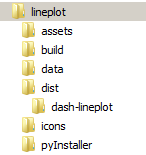
\includegraphics[width=0.3\textwidth]{pic/folderDist}
\caption{Folder structure in bundling \texttt{dash-lineplot.py} with PyInstaller to a distribution folder.
\label{fig:folderdist}}
\end{figure}


The \texttt{dash-lineplot} folder can now be compressed to \texttt{dash-lineplot.zip} and transmitted to the user computer. Installation on the user computer is a simple unzip of the \texttt{zip} file. The user runs the application by opening the folder and launching the \texttt{dash-lineplot} executable by running the \texttt{startPlotTool.bat} script in the top-level folder:

\footnotesize
\begin{lstlisting}
    @echo off

    echo Starting the Dash Line Plot Graphing Tool ....
    echo.
    echo.

    cd dash-lineplot

    if [%1]==[] dash-lineplot.exe
    if not [%1]==[] dash-lineplot.exe --configfile=%1

    set /p DUMMY=done, hit ENTER to exit
\end{lstlisting}
\normalsize

\subsection{Bundling to a single file}

The code can also be bundled to one file:

\footnotesize
\begin{lstlisting}
    pyinstaller --onefile dash-lineplot.py
\end{lstlisting}
\normalsize

In this case \texttt{dash-lineplot.py} script and all its dependencies are bundled into a single executable
named \texttt{dash-lineplot.exe}. One single (very large!) file is distributed to the client.  When started it creates a temporary folder in the appropriate temp-folder location for the operating system. The folder is named \texttt{\_MEIxxxxxx}, where \texttt{xxxxxx} is a random number. The boot loader uncompresses the support files and writes copies into the temporary folder. This can take a little time. That is why a one-file application distribution is slower to start than a one-folder distribution. After creating the temporary folder, the boot loader proceeds exactly
as for the one-folder bundle, in the context of the temporary folder. When the bundled code terminates,
the boot loader deletes the temporary folder.


